\section{Voice Activity Detection} \label{sec:vad}
For the noise PSD estimation in Section \ref{sec:noise_estimation} and the SNR estimation in Section \ref{sec:snr_estimation}, the pressence of speech is needed to increase the performance of the estimators. The Voice Activity Detector will evaluate the frame and give a speechflag wether speech is present or not.

This can be done by looking at the average energy of the frame. In the case of speech present and a SNR bigger than 0, this should be higher than in the case of noise only. To get a linear scaling with respect to the SNR, the log-energy is calculated. We then can express the energy difference as stated in Eq. \ref{eq:TH0} and Eq. \ref{eq:TH1}. This likelihood function is shown in Eq. \ref{eq:vad1} and Eq. \ref{eq:vad2}.

\begin{align}
  T(l) &= \frac{1}{L} \sum_{k=1}^{k=L} log(\Lambda_{k}(l)) \gtreqless_{H_{0}}^{H_{1}} \lambda
  \label{eq:vad1}\\
  \Lambda_{k}(l) &= P_{YY,k}
  \label{eq:vad2}
\end{align}

\begin{align}
  T(l)_{H_{0}}  &\approx  \sigma_{N}^{2}
  \label{eq:TH0}\\
  T(l)_{H_{1}}  &\approx  \sigma_{N}^{2} + SNR
  \label{eq:TH1}
\end{align}

The threshold for the likelihood function could be a constant which is higher than the noise PSD. When noise is dynamic however, this can not be a constant. A dynamic value can be chosen based on the previous noise estimation and SNR estimation. A value between $\sigma_{N}^{2}$ and $\sigma_{N}^{2} + SNR$ can be chosen.

The results of the VAD can be seen in Fig. \ref{fig:VAD}. These results were made using the Noise and SNR estimates from the previous subsystems.

\begin{figure}
  \centering
  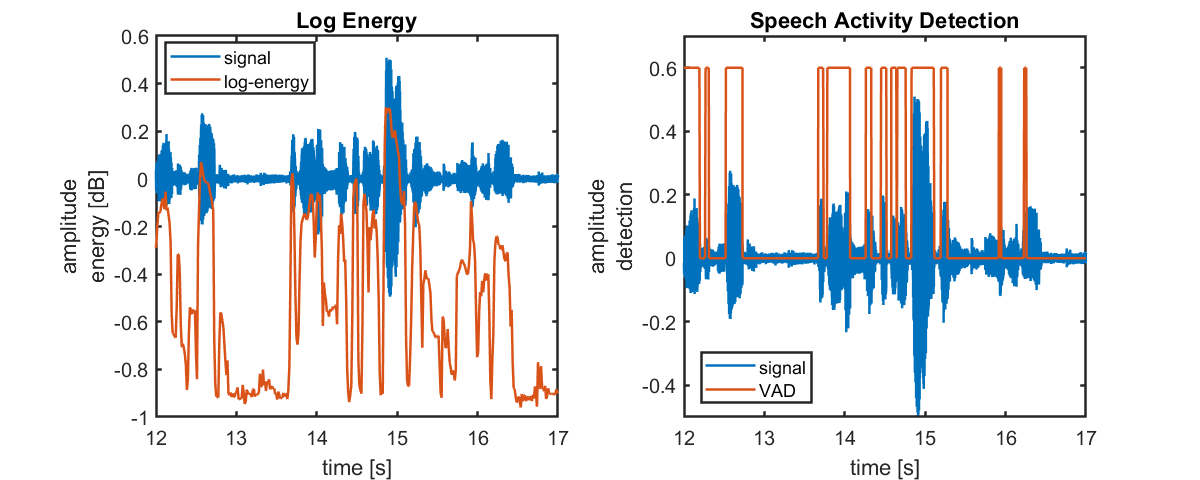
\includegraphics[width=\textwidth]{images/vad.png}
  \caption{Log-energy and VAD performance.}
  \label{fig:VAD}
\end{figure}
